\chapter{Evaluation}\label{Eval}
This chapter is the evaluation of the script based on the Google Lighthouse audit. This chapter will highlight some elements of the audit. The full audit can be seen in appendix \ref{Audit}. The given score in the relevant categories can be seen in figure x. There was a bug in the measurement of the performance score, resulting in a score of 0. The actual score have been manually calculated in the end of section \ref{EvalPerform}. 

\begin{figure} [H]
	\centering
	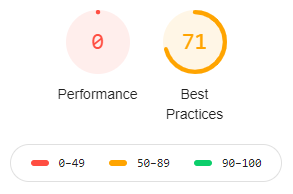
\includegraphics[width=.4\textwidth]{Pictures/LighthouseGrade}
	\caption{The score for performance and best pratices from Google Lighthouse}
	\label{LighthouseGrade}
\end{figure}

\subsection{Performance}\label{EvalPerform}
As shown the performance scored zero out of one hundred. The performance in each of the metrics can be seen in figure \ref{PerformanceAuditValues}.

\begin{figure} [H]
	\centering
	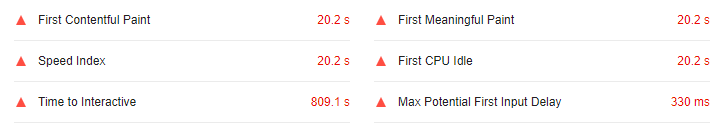
\includegraphics[width=.8\textwidth]{Pictures/PerformanceAuditValues}
	\caption{The result of the performance audit}
	\label{PerformanceAuditValues}
\end{figure}
\fxnote{Remove potential first input delay from figure?}

It does seem like some bug in the tool must have occurred because all of the values are too high. This can be confirmed by comparing with the measurements from the developer tool’s performance tool. These show that the page is fully loaded in 4.6 second, which does not fit with Lighthouse’s 20.2 seconds for First Contentful and First Meaningful Paint. Another sign that something is amiss is the 13.5 minutes before the Time to Interactive, which the tool determined within 10 seconds of analyzing the site. 

Even if the automatic calculation of the performance metrics failed the metrics are still relevant for the evaluation. Using the data from the performance tool these values can be manually estimated. 

\begin{figure} [H]
	\centering
	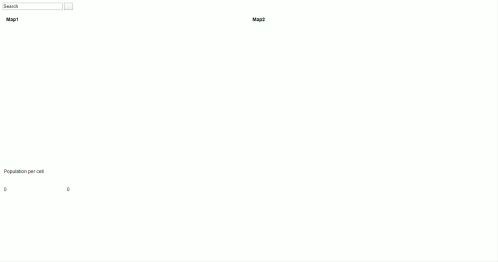
\includegraphics[width=.8\textwidth]{Pictures/ScreenshotLoading1}
	\caption{After 0.3 seconds the search bar and legend appears.}
	\label{ScreenshotLoading1}
\end{figure}

Figure x, x and x are all screenshots of the website taken by the performance tool, while the page was loading. The maps are not utilising the full screen extent as mentioned in section \ref{DTTwoMaps}, which is the reason for the empty white space next to the maps. Figure x is taken 0.3 seconds after the page started loading. This time is both the First Meaningful Paint and First CPU Idle since the user can interact with the searchbar.

\begin{figure} [H]
	\centering
	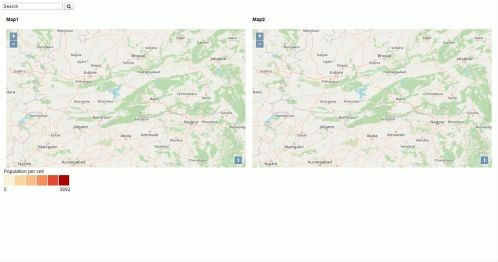
\includegraphics[width=.8\textwidth]{Pictures/ScreenshotLoading2}
	\caption{After 1 second the map appears without the raster layer}
	\label{ScreenshotLoading2}
\end{figure}

After 1 second the maps appear on the website as shown in figure x. The user is able pan and zoom in the map, so this is the Time to Interactive. 

\begin{figure} [H]
	\centering
	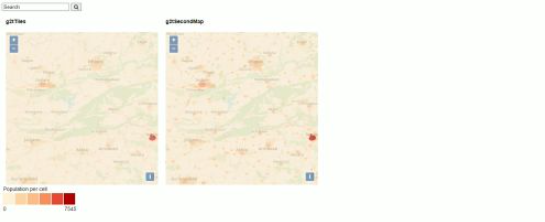
\includegraphics[width=.8\textwidth]{Pictures/ScreenshotLoading3}
	\caption{After 3.6 seconds the map is fully loaded}
	\label{ScreenshotLoading3}
\end{figure}

The last screenshot at figure x shows the map fully loaded after 3.6 seconds. With the tiff tiles being loaded and visualized this is the time for the First Meaningful Paint. This can be used as a conservative estimate for the Speed Index. This would be the value for the Speed Index if everything got visualized at this time and nothing had been visualized on the website prior.

The real Speed Index would be lower, since the legend, map titles and search bar have been visualized at an earlier stage. 

These metrics can then manually be calculated into a score using the Lighthouse Scoring Calculator as shown in figure x. The calculator in unable to take inputs below 1 second. Based on the given value the performance should have scored 94. This score will be discussed upon in section \ref{label}
https://googlechrome.github.io/lighthouse/scorecalc/

\begin{figure} [H]
	\centering
	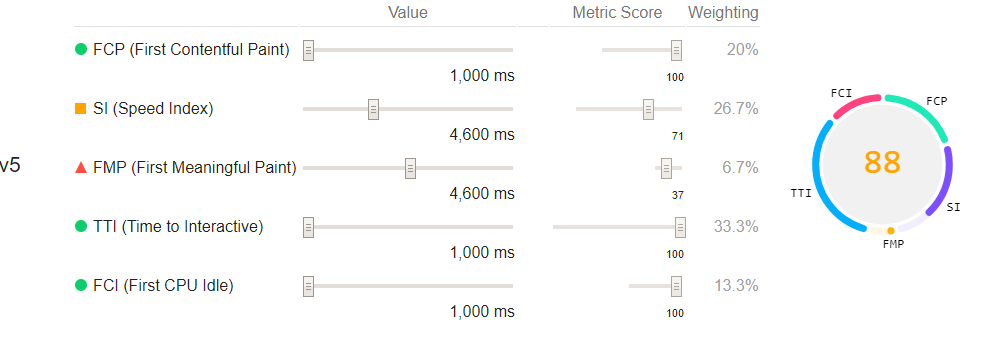
\includegraphics[width=.9\textwidth]{Pictures/ScoringManual}
	\caption{The website for manually calculating the scores, which Lighthouse grants}
	\label{ScoringManual}
\end{figure}

\fxnote{They say themself, that scoring 0 repeaedly usually indicate an error - Lighthouse}

\subsection{Opportunities}
In addition to providing the metrics for the performance Lighthouse also comes with suggestion to how the loading time can be reduced. In this subsection only some of these will be preset. The rest can be seen in appendix \ref{Audit}.

\textbf{Eliminate render-blocking resources}\\
The opportunity for the largest estimated time saving is to eliminate render-blocking resources. These are the URLs, which must be loaded before the first paint can be applied to the page. \citep{RenderBlocking}

The largest render-blocking resource is Openlayers, which at 2784 kB makes up 82 \% of the blocking resources. When analysed further with the Coverage tool in the dev tools it can be seen that 42.7 \% of the Openlayers library is not being used. The performance could therefore be improved by only loading the necessary parts of the library. The size of it could also be reduced by using the minified version of it instead of the debug-version.


\fxnote{Lad være med at tage alle argumenterne med og skriv i starten at ikke alt er med}
 
\fxnote{Have I written about Jquery??}

\fxnote{Have I explained the difference between HTTP 1 and 2?}

 
\fxnote{søg på Http}
\fxnote{Write about Coverage earlier – maybe in evaluation tools}

%\textbf{Minification and compressing}\\
%Files sizes and script parsing time can be reduced by minifying and compressing the files. 
%
%A minified file is a file, where all the unnecessary parts have been cut away. Whitespaces and unused code are removed leaving a smaller file, which still functions perfectly. 
%
%Compression is using an algorithm to modify the data, so that it takes up less space.
%\citep{MinifyJS}

\textbf{Avoid enormous network payloads}\\
Long loading times are highly correlated with the amount of loaded data.  
\citep{LoadingTooMuch}

Loading the raster tiles for the map does require loading multiple files with a large bit depth, which requires a lengthy loading time. The amount of loaded tiles could be reduced, if the issue coursing tiles from the wrong layer to be loaded got fixed. A potential course to this issue is presented in section \ref{WhyWrongLevel}.

\textbf{Does not use HTTP/2 for all of its resources}\\
This suggested improvement appears if some of the page’s resources are being served with a version of HTTP/1. According to Google Audit all loaded resources are being delivered using HTTP 1.1.
\citep{HTTP2}

This was the suggestion, which lead to replacing initial testing server with a Caddy test server, which vastly reduced the load time as illustrated in figure \ref{CaddyVsPython}.

\begin{figure} [H]
	\centering
	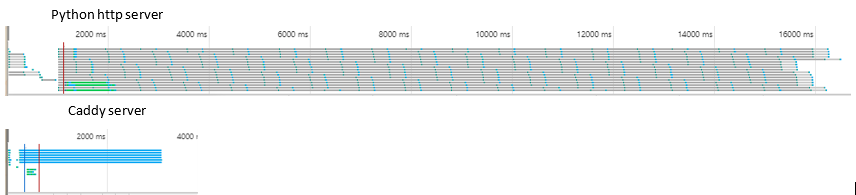
\includegraphics[width=1\textwidth]{Pictures/CaddyVsPython}
	\caption{Screenshot of the network connection for a python and a caddy server}
	\label{CaddyVsPython}
\end{figure}

Figuren is two screenshots from the network tab of Chromes developer tool when the page is served with a python server (top) and caddy server (bottom). 
The grey bars are when a loaded file is being stalled. The blue bars are when they are loaded. This figure shows that the serving is being optimized, where the stalling largely is gone. 

However even after setting up Caddy the error message was still present. It is uncertain if this means that the connection still is HTTP/1 based or if it is HTTP/2 but labelled incorrectly. 


\fxnote{Mention caddy – 6 connection issue earlier}
\fxnote{Remember to add the source behind the bar colors here - it is here now, but is invisible}

%https://developers.google.com/web/tools/chrome-devtools/network/reference?utm_source=devtools#timing-explanation


\fxnote{Write about HTTP/2 earlier?}



\textbf{Uses deprecated APIs}\\
When loading the metadata about the tiles a synchronous XMLRequest is used. This is a deprecated API, which will be removed from Chrome in a feature edition. This should be rewritten as an asynchronous request instead.
\citep{OldApis}
\fxnote{borgerinddragelses værktøj}


\section{Postload performance}

In addition to the measurements of the performance for loading the site the performance after loading was also measured. In table \ref{tabPostloadPerformance} is measurements of performance of using the tool. It can be seen that loading and coloring a new layer takes 3.89 seconds, whereas coloring a layer, which already have been loaded takes on average 0.56 seconds. 

\begin{table}[htbp]
	\centering
	\begin{tabular}{l}
		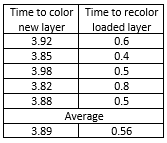
\includegraphics[width=0.3\textwidth]{Pictures/tabPostloadPerformance}
	\end{tabular}
	\caption{Seconds to load a new layer and color it and to recolor a loaded layer}
	\label{tabPostloadPerformance}
\end{table}